%%%%%%%%%%%%%%%%%%%%%%%%%%%%%%%%%%%%%%%%%%%%
\section{Appendix}

\begin{frame}
  \frametitle{Table of Contents}
  \tableofcontents[currentsection]
\end{frame}


\subsection{I: Fetal Poses, II: Fetal Behaviours}

%%%%%%%%%%%%%%%%%%%%%%%%%%%%%%%%%%%%%%%%%%%%%%%%%%%%%%%%
{
\paper{Ferguson and Haultain 1889 in Handbook of Obstetric Nursing, pages 150–153; Mori et al. 2010 in ICDL}
\begin{frame}{I: Fetal Poses, II: Fetal Behaviours}
      \begin{figure}
        \centering
        \includegraphics[width=1.0\textwidth]{fetal-poses/versions/drawing-v01.png}
        %\caption{}
      \end{figure}
\end{frame}
}

\subsection{Growing Baby: 3D Print-ready Models}


%%%%%%%%%%%%%%%%%%%%%%%%%%%%%%%%%%%%%%%%%%%%%%%%%%%%%%%%
{
\paper{Growing Baby: 3D Print-ready Models}
\begin{frame}{III: Fetal Growth}
      \begin{figure}
        \centering
        \includegraphics[width=1.0\textwidth]{fetal-ages/versions/drawing-v02.png}
        %\caption{}
      \end{figure}
\end{frame}
}


\subsection{State-of-the-art on modelling fetus}

%%%%%%%%%%%%%%%%%%%%%%%%%%%%%%%%%%%%%%%%%%%%%%%%%%%%%%%%
{
%\paper{Wright-Gilbertson M. 2014 in PhD thesis}
\begin{frame}{State-of-the-art on modelling fetus}
      \begin{figure}
        \centering
        \includegraphics[width=1.0\textwidth]{state-of-the-art/versions/drawing-v01}
        %\caption{}
      \end{figure}
\end{frame}
}




% %%%%%%%%%%%%%%%%%%%%%%%%%%%%%%%%%%%%%%%%%%%%%%%%%%%%%%%%
% {
% %\paper{Wright-Gilbertson M. 2014 in PhD thesis}
% \begin{frame}{Fetal Biomechanics}
%       \begin{figure}
%         \centering
%         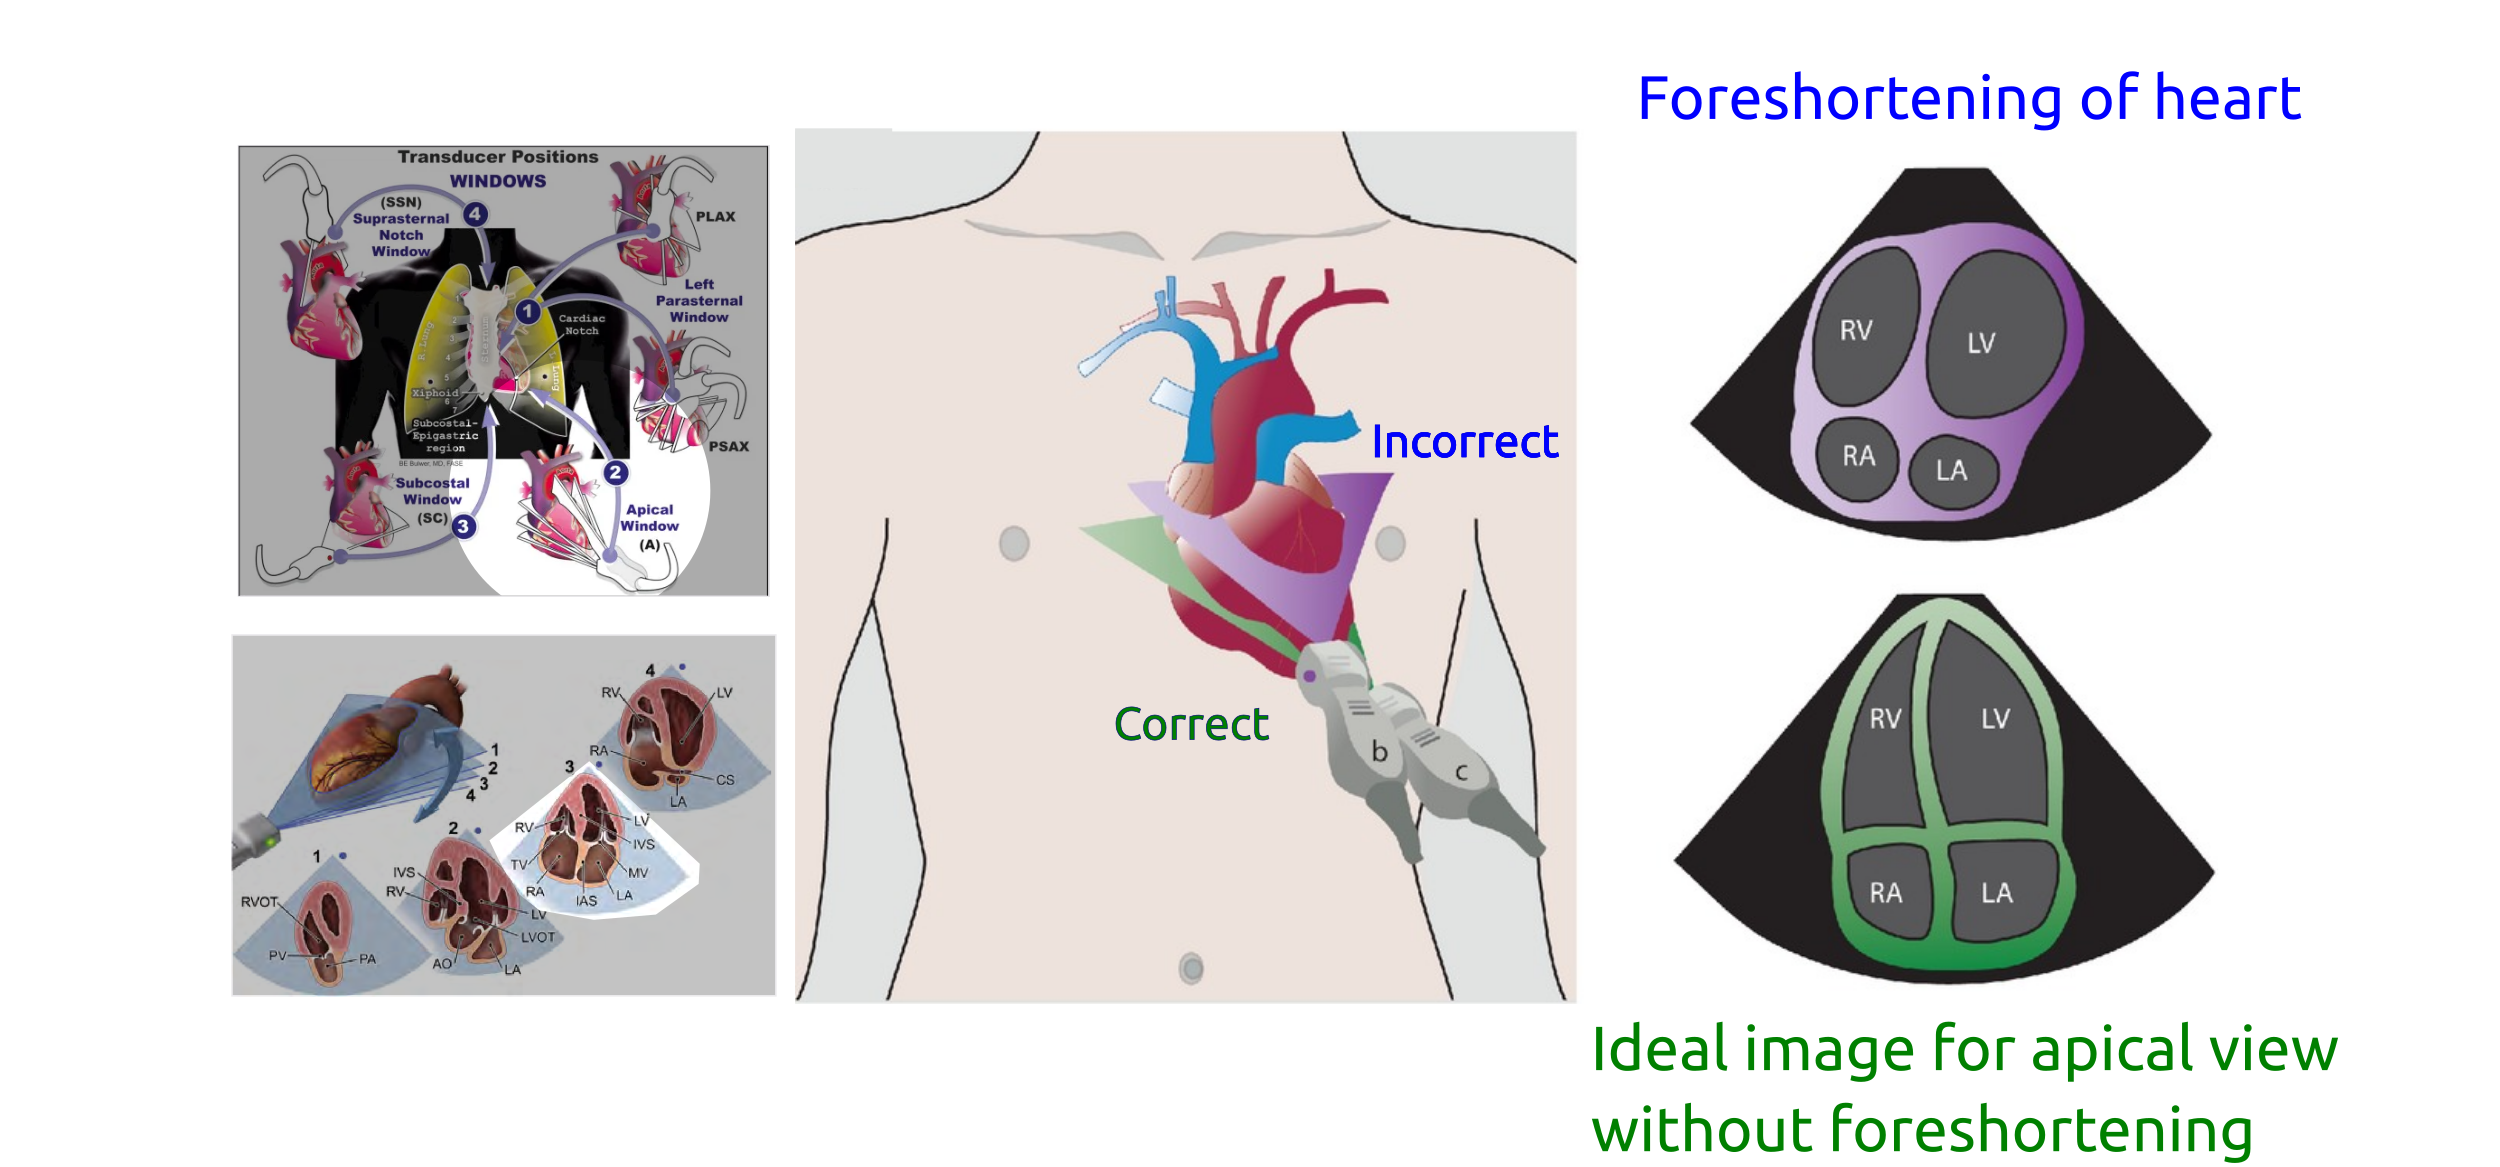
\includegraphics[width=1.0\textwidth]{fetal-biomechanics/versions/drawing-v00.png}
%         %\caption{}
%       \end{figure}
% \end{frame}
% }


% %%%%%%%%%%%%%%%%%%%%%%%%%%%%%%%%%%%%%%%%%%%%%%%%%%%%%%%%
% {
% %\paper{(a) Coordinate systems overview sketch in 3D Slicer,  (b) Asselin et al. 2018 in conf-BIVPCS, (c) US-simulator, and (d) 3D-printed fetus}
% %\paper{}
% \begin{frame}{Challenges of the fellowship}


%       \begin{figure}
%         \centering
%         \includegraphics[width=1.0\textwidth]{simulator-for-ugi/versions/drawing-v02.png}
%       \end{figure}


% \end{frame}
% }




%%%%BLURS

% %%%%%%%%%%%%%%%%%%%%%%%%%%%%%%%%%%%%%%%%%%%%
% \subsection{Research Questions}


% %%%%%%%%%%%%%%%%%%%%%%%%%%%%%%%%%%%%%%%%%%%%%%%%%%%%%%%%
% {
% %\paper{Wright-Gilbertson M. 2014 in PhD thesis}
% \begin{frame}{Research Questions}	
%  %Can we understand more about fetal development trough the development of more realistic phantoms
% %Can dynamic fetal phantoms be created to understand fetal development?  %added Thu 15 Apr 05:20:09 BST 2021
% %Can synthetic fetus help to understand fetal development? %Fri 23 Apr 05:56:53 BST 2021
% %* Can the creation of synthetic fetuses help to understand fetal development? %Wed 12 May 08:20:58 BST 2021 
% %* Can the creation of synthetic fetuses predict fetal development issues? %Wed 12 May 09:50:47 BST 2021

% \BigSizeFont
% \begin{itemize}
% %\item Would the creation of synthetic fetuses help to understand 
% %the biomechatincs of phetal development? %Sat 15 May 14:51:42 BST 2021
% %\item Can we understand fetal development with synthetic fetuses? %Sat 15 May 15:08:19 BST 2021
% %\item Can the understanding of fetal biomechanics lead to predict fetal pathologies? %Mon 12 Jul 09:25:41 BST 2021
% % MORE ON FETAL PATHOLOGIES:https://www.sciencedirect.com/topics/medicine-and-dentistry/fetal-pathology
% \item Can fetal biomechanics help to understand the prediction of fetal pathologies? %% Mon 12/07/2021 09:45
% \item Would AI-based fetal biomechanics automatically predict fetal pathologies? %Tue 19 Oct 16:54:45 BST 2021
% \item \end{itemize}

% \end{frame}
% }


%\subsection{State-of-the-art on modelling fetus}


